% Opsætter KU Tex dokument
%%%%%%%%%%%%%%%%%%%%%%%%%%%%%%%%%%%%%%%%%%%%%%%%%%%%%%%%%%%%%%%%%%%%%%%%%%%%%%%%
\documentclass{article}                                                        %
\usepackage[a4paper, hmargin={2.8cm, 2.8cm}, vmargin={2.5cm, 2.5cm}]{geometry} %
\usepackage{eso-pic}  % \AddToShipoutPicture                                   %
\usepackage{graphicx} % \includegraphics                                       %
%\usepackage{subfig} - Can not be used with subcaption package (for subfigures)
\usepackage{setspace}                                                        %
%%%%%%%%%%%%%%%%%%%%%%%%%%%%%%%%%%%%%%%%%%%%%%%%%%%%%%%%%%%%%%%%%%%%%%%%%%%%%%%%

% Pakker til skrifttyper, tekst osv.
%%%%%%%%%%%%%%%%%%%%%%%%%%%%%%%%%%%%%%%%%%%%%%%%%%%%%%%%%%%%%%%%%%%%%%%%%%%%%%%%
    \usepackage[utf8]{inputenc}  % Implementere Unicode                        %
    \usepackage[T1]{fontenc}     % Unicode skrifttype fx. é skrives som 1 tegn %
    \usepackage[english]{babel}   % Dansk Ordbog                                %
    \usepackage{microtype}       % Forbedre linjeombrydningen                  %
    \usepackage{libertine}       % Skrifttype                                  %
%%%%%%%%%%%%%%%%%%%%%%%%%%%%%%%%%%%%%%%%%%%%%%%%%%%%%%%%%%%%%%%%%%%%%%%%%%%%%%%%

% Pakker til matematik og kode.
%%%%%%%%%%%%%%%%%%%%%%%%%%%%%%%%%%%%%%%%%%%%%%%%%%%%%%%%%%%%%%%%%%%%%%%%%%%%%%%%
    \usepackage{mathtools}       % Udvidelse til amsmath pakken                %
    \usepackage{amsthm}          % Pakke til bevisførelse                      %
    \usepackage{amssymb}         % Extra matematiske symboler                  %				
	\usepackage{mychemistry}												   %
	\usepackage[version=3]{mhchem}											   %
	\usepackage{wrapfig}													   %
	\usepackage{siunitx}	
	\usepackage{anyfontsize}
	\usepackage{ragged2e}
	\usepackage{algorithm2e}
	\usepackage[final]{pdfpages}
	\usepackage{listings}
	\usepackage{tikz}
	\usepackage{multirow}
	\usepackage{makecell}
	\usepackage{fourier} 
	\usepackage{array}
	\usepackage{todonotes}
	\usepackage{pdflscape}
	\usetikzlibrary{arrows,shapes}
	\usepackage{titlesec}
	\usepackage{hyperref}
	\usepackage{url}
	\usepackage[nottoc,numbib]{tocbibind}
	\usepackage{semantic}
	\usepackage{subcaption}
	\usepackage{qtree}
	
	\definecolor{light-gray}{gray}{0.85}
	\lstset{
	    	numbers=left,
	    	breaklines=true,
	    	backgroundcolor=\color{light-gray},
	    	tabsize=2,
	    	basicstyle=\ttfamily,
	    	literate={\ \ }{{\ }}1
	}
	
	\urlstyle{same}
	\tikzstyle{vertex}=[circle,fill=white!25,minimum size=20pt,inner sep=0pt]
	\tikzstyle{edge} = [draw,thick,-]

	\definecolor{light-gray}{gray}{0.85}
	\definecolor{dkgreen}{RGB}{0.0,128.0,43.0}
	\lstdefinelanguage{FSharp}%
{morekeywords={new, match, with, rec, open, module, namespace, type, of, member, % 
and, for, while, true, false, in, do, begin, fun, function, return, yield, try, %end
mutable, if, then, else, cloud, async, static, use, abstract, interface, inherit, finally, int },
  otherkeywords={ let!, return!, do!, yield!, use!, var, from, select, where, order, by },
  keywordstyle=\color{bluekeywords},
  sensitive=true,
  basicstyle=\ttfamily,
	breaklines=true,
  xleftmargin=\parindent,
  aboveskip=\bigskipamount,
	tabsize=4,
  morecomment=[l][\color{dkgreen}]{///},
  morecomment=[l][\color{dkgreen}]{//},
  morecomment=[l][\color{dkgreen}]{(*},
  morecomment=[s][\color{dkgreen}]{},
  morestring=[b]",
  showstringspaces=false,
  literate={`}{\`}1,
  stringstyle=\color{redstrings},
}
	
	
												   %
%%%%%%%%%%%%%%%%%%%%%%%%%%%%%%%%%%%%%%%%%%%%%%%%%%%%%%%%%%%%%%%%%%%%%%%%%%%%%%%%

% Pakker til layout.
%%%%%%%%%%%%%%%%%%%%%%%%%%%%%%%%%%%%%%%%%%%%%%%%%%%%%%%%%%%%%%%%%%%%%%%%%%%%%%%%
    \usepackage{fancyhdr}            % Gør det muligt at bruge sidehoveder     %
    \usepackage{graphicx}            % Mulighed for bl.a. \includegraphics     %
    \usepackage{colortbl}            % Hvis man vil farvelægge sine tabeller   %
    \usepackage{array}               % Gør miljøerne array og tabular bedre    %
    \usepackage{parskip}             % Første paragraf i afsnit indrykkes ikke %
    \usepackage{titlesec}            % Tilpassing af afstand mellem sektioner  %
    \usepackage[lastpage,user]{zref} % Side x af y                             %
%%%%%%%%%%%%%%%%%%%%%%%%%%%%%%%%%%%%%%%%%%%%%%%%%%%%%%%%%%%%%%%%%%%%%%%%%%%%%%%%


% Implementerer en række makroer og de pakker der er importeret
%%%%%%%%%%%%%%%%%%%%%%%%%%%%%%%%%%%%%%%%%%%%%%%%%%%%%%%%%%%%%%%%%%%%%%%%%%%%%%%%
    \pagestyle{fancy}                        % Implementerer sidehoved         %
    \lhead{University of Copenhagen}                % Venstre sidehoved               %
    \rhead{Casper Bresdahl}                             % Højre sidehoved      %
    \cfoot{\thepage\ of \zpageref{LastPage}} % Side x af y                     %
    \newtheorem*{prp}{Propostion}            % Skaber nyt theorem  
    \renewcommand{\baselinestretch}{1.25}       %
%%%%%%%%%%%%%%%%%%%%%%%%%%%%%%%%%%%%%%%%%%%%%%%%%%%%%%%%%%%%%%%%%%%%%%%%%%%%%%%%

% Mindsker afstanden mellem sektioner
%%%%%%%%%%%%%%%%%%%%%%%%%%%%%%%%%%%%%%%%%%%%%%%%%%%%%%%%%%%%%%%%%%%%%%%%%%%%%%%%%%
\titlespacing\section{0pt}{12pt plus 4pt minus 2pt}{0pt plus 1pt minus 3pt}      %
\titlespacing\subsection{0pt}{12pt plus 4pt minus 2pt}{0pt plus 1pt minus 3pt}   %
\titlespacing\subsubsection{0pt}{12pt plus 4pt minus 2pt}{0pt plus 1pt minus 3pt}%
%%%%%%%%%%%%%%%%%%%%%%%%%%%%%%%%%%%%%%%%%%%%%%%%%%%%%%%%%%%%%%%%%%%%%%%%%%%%%%%%%%

%Ændrer størelsen på sections
%%%%%%%%%%%%%%%%%%%%%%%%%%%%%%%%%%%%%%%%%%%%%%%%%%%%%%%%%%%%%%%%%%%%%%%%%%%%%%%%%%
\titleformat{\section}
{\normalfont\fontsize{14}{16}\bfseries}{\thesection}{1em}{}
\titleformat{\subsection}
{\normalfont\fontsize{12}{14}\bfseries}{\thesubsection}{1em}{}
\titleformat{\subsubsection}
{\normalfont\fontsize{11}{13}\bfseries}{\thesubsubsection}{1em}{}
%%%%%%%%%%%%%%%%%%%%%%%%%%%%%%%%%%%%%%%%%%%%%%%%%%%%%%%%%%%%%%%%%%%%%%%%%%%%%%%%%%

%%%%%%%%%%%%
% Document %
%%%%%%%%%%%%

\begin{document}

\begin{titlepage}

\newcommand{\HRule}{\rule{\linewidth}{0.5mm}} % Defines a new command for the horizontal lines, change thickness here

\begin{center}
 % Center everything on the page
 
%----------------------------------------------------------------------------------------
%	HEADING SECTIONS
%----------------------------------------------------------------------------------------

\textsc{\LARGE University of Copenhagen}\\[1.5cm] % Name of your university/college
\textsc{\Large Computer Science}\\[0.5cm] % Major heading such as course name
\textsc{\large Signal and Image Processing}\\[0.5cm] % Minor heading such as course title

%----------------------------------------------------------------------------------------
%	TITLE SECTION
%----------------------------------------------------------------------------------------

\HRule \\[0.4cm]
{ \huge \bfseries Assignment 4}\\[0.4cm] % Title of your document
\HRule \\[1.5cm]
 
%----------------------------------------------------------------------------------------
%	AUTHOR SECTION
%----------------------------------------------------------------------------------------

\begin{minipage}{0.4\textwidth}
\begin{flushleft} \large
\emph{Author:}\\ 
% Your name
Casper \textsc{Bresdahl} \\
\hfill
\end{flushleft}
\end{minipage}
~
\begin{minipage}{0.4\textwidth}
\begin{flushright} \large
\emph{Teachers:} \\
Kim \textsc{Pedersen}\\
Sune \textsc{Darkner}
\end{flushright}
\end{minipage}\\[2cm]

% If you don't want a supervisor, uncomment the two lines below and remove the section above
%\Large \emph{Forfattere:}\\
%Axel \textsc{Christof}\\% Your name
%Casper \textsc{Bresdahl}\\
%Emilie \textsc{Bentsen}\\[1cm] 

%----------------------------------------------------------------------------------------
%	DATE SECTION
%----------------------------------------------------------------------------------------

{\large \today}\\[2cm] % Date, change the \today to a set date if you want to be precise

%----------------------------------------------------------------------------------------
%	LOGO SECTION
%----------------------------------------------------------------------------------------


\includegraphics{logo.png}\\[1cm] % Include a department/university logo - this will require the graphicx package
 
%----------------------------------------------------------------------------------------

\vfill % Fill the rest of the page with whitespace

%Disse linjer skaber forside, evt indholdsfortegnelse, og sætter sidetal
%%%%%%%%%%%%%%%%%%%%%%%%%%%%%%%%%%%%%%%%%%%%%%%%%%%%%%%%%%%%%%%%%%%%%%%%%%%%%%%%
									                                           %
    \thispagestyle{empty}   % Fjerner sidetal forside                          %
        % Slå disse til hvis der ønskes indholdsfortegnelse                    %
        %%%%%%%%%%%%%%%%%%%%%%%%%%%%%%%%%%%%%%%%%%%%%%%%%%%%%%%%%%%%%%%%%%%%%%%% 
            \newpage                % Side til indholdsfortegnelse            %
            %\thispagestyle{empty}   % Fjerner sidetal fra indholdsfortegnelse %
            %\tableofcontents        % Skaber indholdsfortegnelse              %
    \end{center}
    %\section*{Forord}
    	
		
        %%%%%%%%%%%%%%%%%%%%%%%%%%%%%%%%%%%%%%%%%%%%%%%%%%%%%%%%%%%%%%%%%%%%%%%%
    \newpage                % Første rigtige side
    \setcounter{page}{1}    % Sætter rigtigt sidetal på første side
%%%%%%%%%%%%%%%%%%%%%%%%%%%%%%%%%%%%%%%%%%%%%%%%%%%%%%%%%%%%%%%%%%%%%%%%%%%%%

\end{titlepage}
{\fontsize{10}{14}\selectfont

\section{Exercise 1}
\subsection*{1.1}
When performing correlation and convolution we look at each pixel in the image at turn. The 'x' filter in this exercise looks at the pixel to the right and weights it by $1/2$, it looks at the pixel to the left and weights it $-1/2$, but the center pixel is not apparent in the formula, and is thus weighted zero. The same goes for the 'y' filter of the exercise. Thus we have:\\ 
'x' filter for convolution:	\begin{tabular}{|l|l|l|}
	\hline
	1/2 & 0 & -1/2 \\ \hline
\end{tabular}\\
'x' filter for correlation: \begin{tabular}{|l|l|l|}
	\hline
	-1/2 & 0 & 1/2 \\ \hline
\end{tabular}\\
'y' filter for convolution: \begin{tabular}{|l|}
		\hline
		1/2  \\ \hline
		0    \\ \hline
		-1/2 \\ \hline
	\end{tabular}\\
'y' filter for correlation: \begin{tabular}{|l|}
	\hline
	-1/2  \\ \hline
	0    \\ \hline
	1/2 \\ \hline
\end{tabular}\\
For all the filters the center pixel is the zero in the kernel. There is no difference between correlation and convolution if the kernel is symmetric. Given a Gaussian kernel is symmetric and a mean filter is constant (and thus also symmetric) there is no difference between convolution and correlation with these filters.

\subsection*{1.2}
Linearly separating the Sobel y derivative filter gives us:\\
\begin{equation*}
	f*\begin{bmatrix}
		1&2&1\\
		0&0&0\\
		-1&-2&-1
	\end{bmatrix}
 = f*\begin{bmatrix}
 	1\\
 	0\\
 	-1
 \end{bmatrix}
* \begin{bmatrix}
	1&2&1
\end{bmatrix}
\end{equation*}
Linearly separating the Prewitt y derivative filter gives us:\\
\begin{equation*}
	f*\begin{bmatrix}
		1&1&1\\
		0&0&0\\
		-1&-1&-1
	\end{bmatrix}
	= f*\begin{bmatrix}
		1\\
		0\\
		-1
	\end{bmatrix}
	* \begin{bmatrix}
		1&1&1
	\end{bmatrix}
\end{equation*}
We see that the separated y filter is almost identical to the one from the previous exercise, that is, we get almost the same result when convolving with the y filter alone. But for the Sobel and Prewitt filters we also convolve with an x filter afterwards, this means we involve more pixels in the convolution, and 'smooth' the noise more. We can look at the x filter as a 'smoothing' filter, as we are smoothing the image afterwards by adding the neighbouring pixel values to the center pixel. Because we involve more pixels in the convolution, the noisy pixels gets weighted less in total.

\subsection*{1.3}
\begin{figure}[H]
	\centering
	\begin{subfigure}[b]{\textwidth}
		\centering
		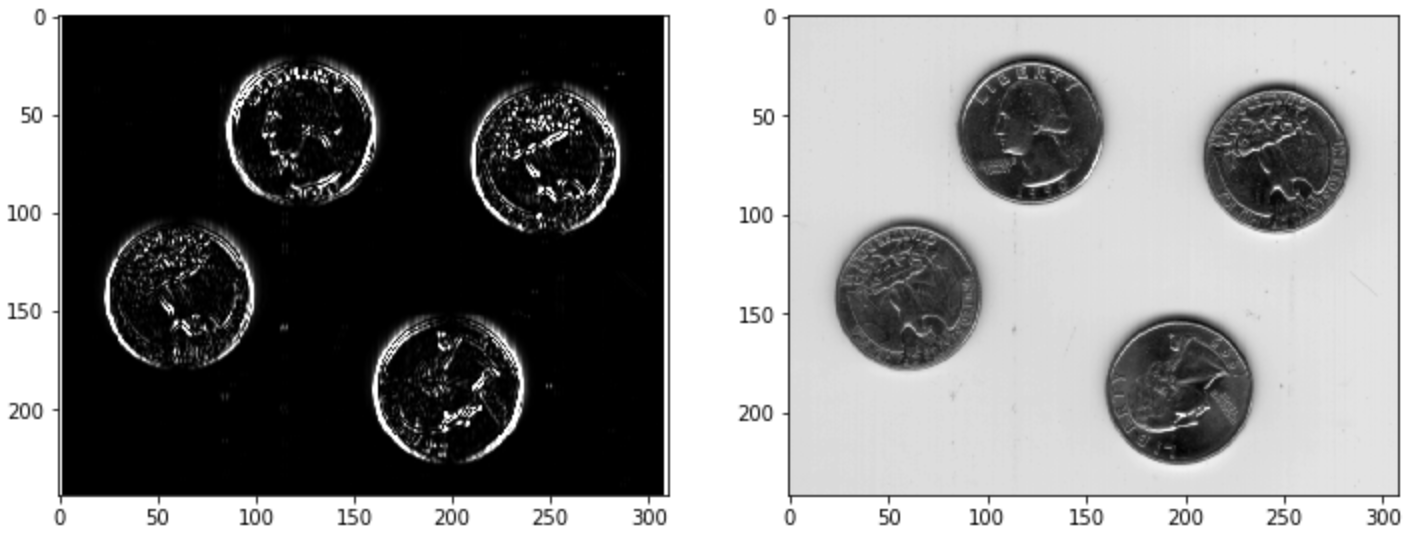
\includegraphics[width=\textwidth]{Materials/svar0}
		\caption{Variance 0}
	\end{subfigure}
	\hfill
	\\
	\begin{subfigure}[b]{\textwidth}
		\centering
		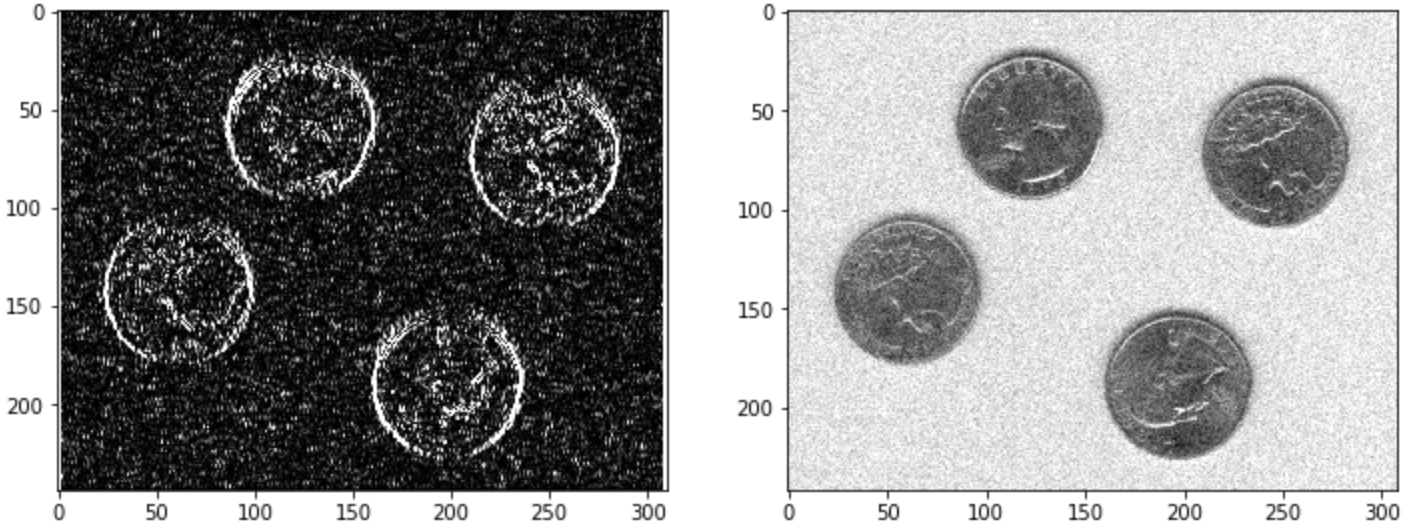
\includegraphics[width=\textwidth]{Materials/svar005}
		\caption{Variance 0.005}
	\end{subfigure}
	\hfill
	\\
	\begin{subfigure}[b]{\textwidth}
		\centering
		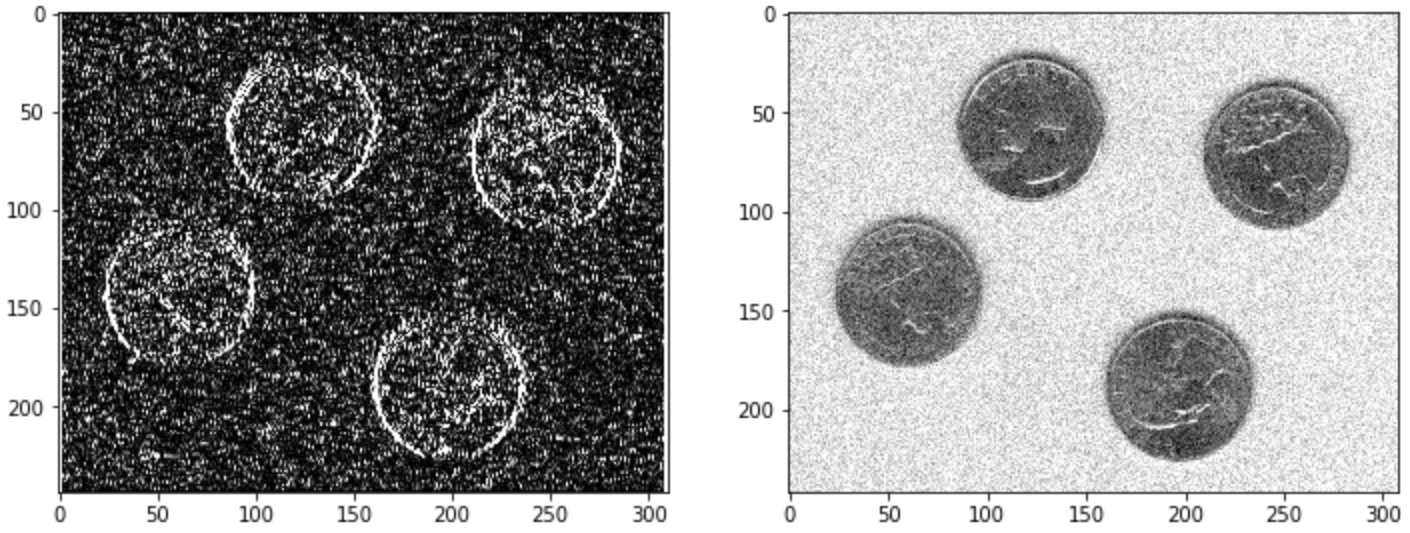
\includegraphics[width=\textwidth]{Materials/svar01}
		\caption{Variance 0.01}
	\end{subfigure}
	\caption{Gradients produced by filtering with Sobel.}
	\label{sobel1}
\end{figure}
\begin{figure}[H]
	\centering
	\begin{subfigure}[b]{0.85\textwidth}
		\centering
		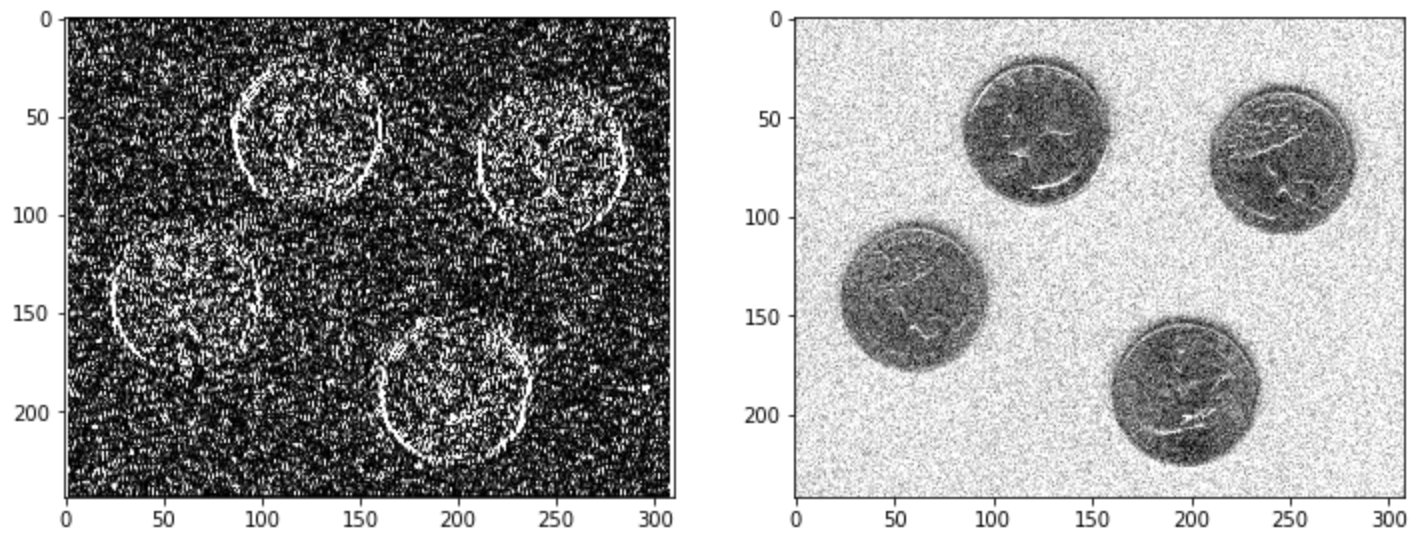
\includegraphics[width=\textwidth]{Materials/svar015}
		\caption{Variance 0.015}
	\end{subfigure}
	\hfill
	\\
	\begin{subfigure}[b]{\textwidth}
		\centering
		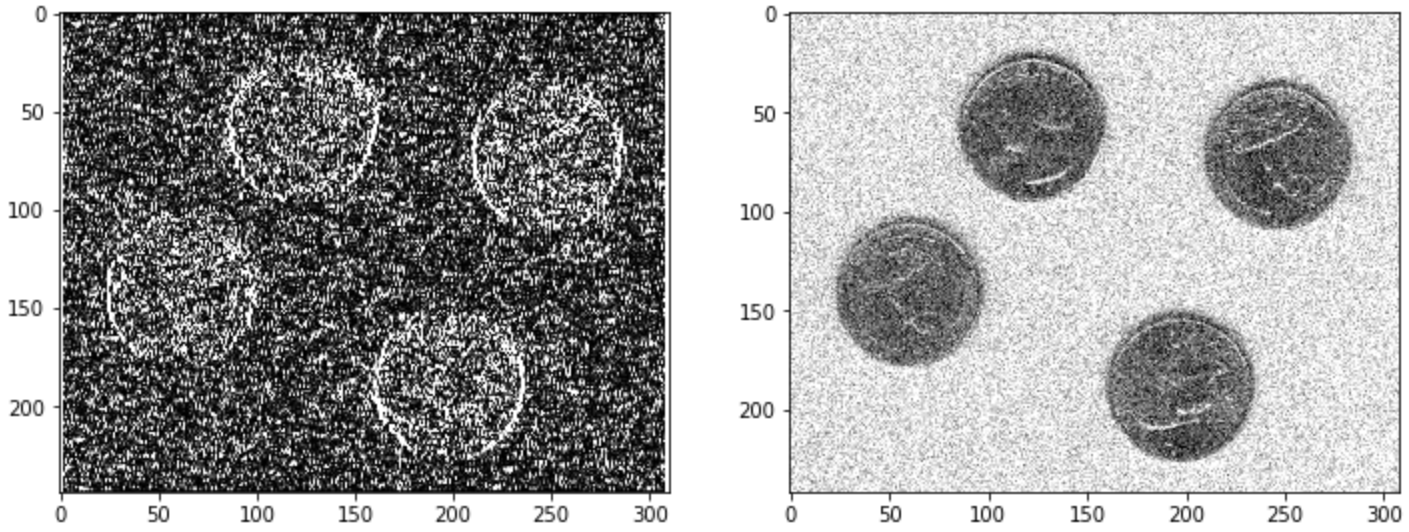
\includegraphics[width=0.85\textwidth]{Materials/svar02}
		\caption{Variance 0.02}
	\end{subfigure}
	\caption{Gradients produced by filtering with Sobel.}
	\label{sobel2}
\end{figure}

\begin{figure}[H]
	\centering
	\begin{subfigure}[b]{0.85\textwidth}
		\centering
		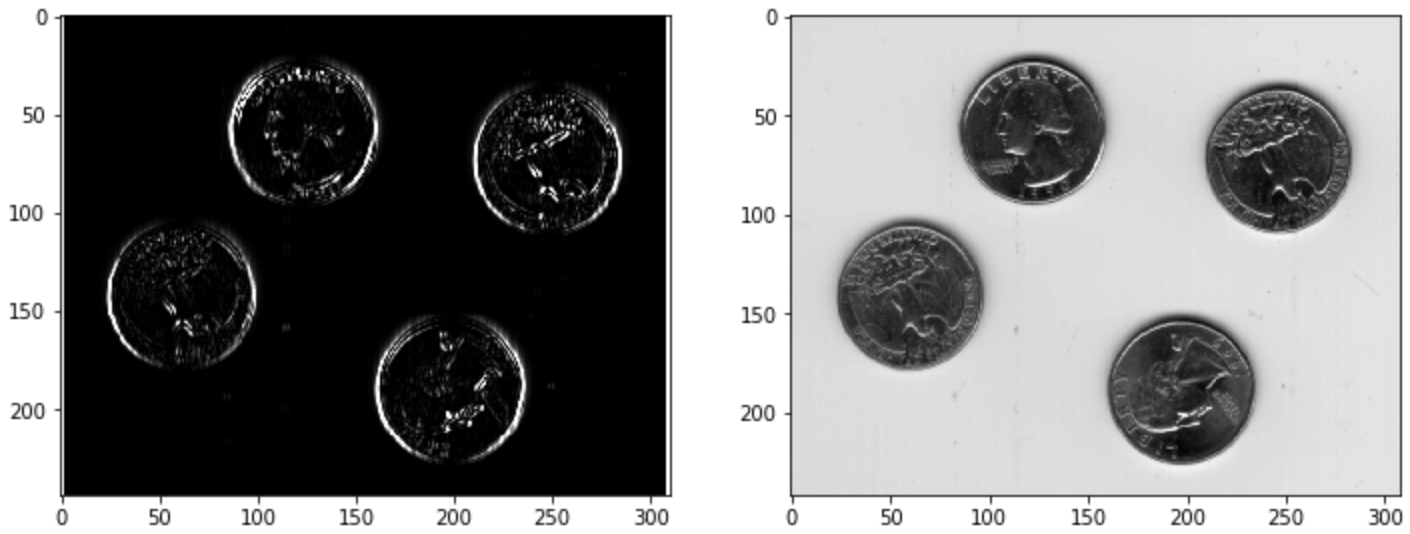
\includegraphics[width=\textwidth]{Materials/pvar0}
		\caption{Variance 0}
	\end{subfigure}
	\hfill
	\\
	\begin{subfigure}[b]{0.85\textwidth}
		\centering
		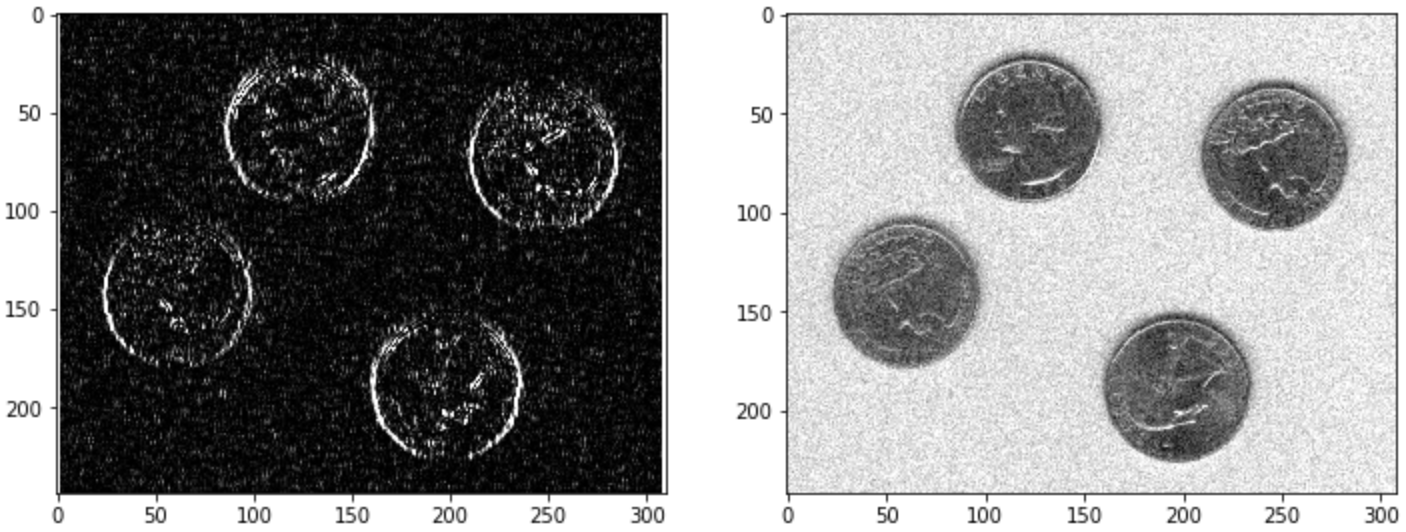
\includegraphics[width=\textwidth]{Materials/pvar005}
		\caption{Variance 0.005}
	\end{subfigure}
	\caption{Gradients produced by filtering with Prewitt.}
	\label{prewitt1}
\end{figure}
\begin{figure}[H]
	\centering
		\begin{subfigure}[b]{\textwidth}
		\centering
		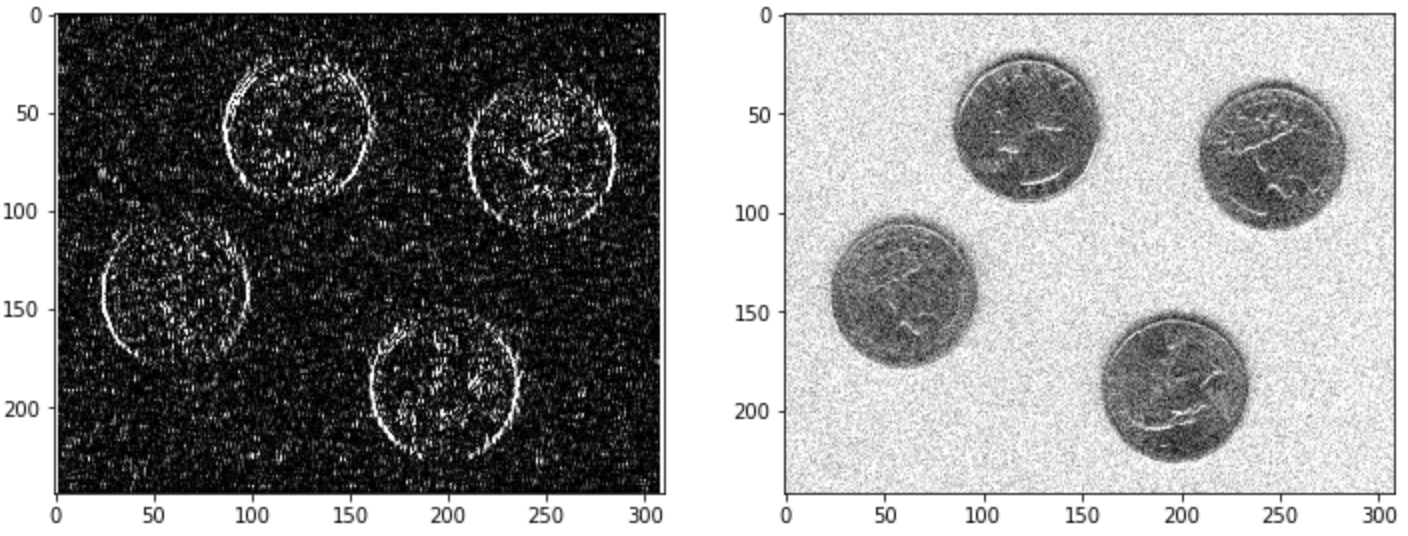
\includegraphics[width=\textwidth]{Materials/pvar01}
		\caption{Variance 0.01}
	\end{subfigure}
	\hfill
	\\
	\begin{subfigure}[b]{\textwidth}
		\centering
		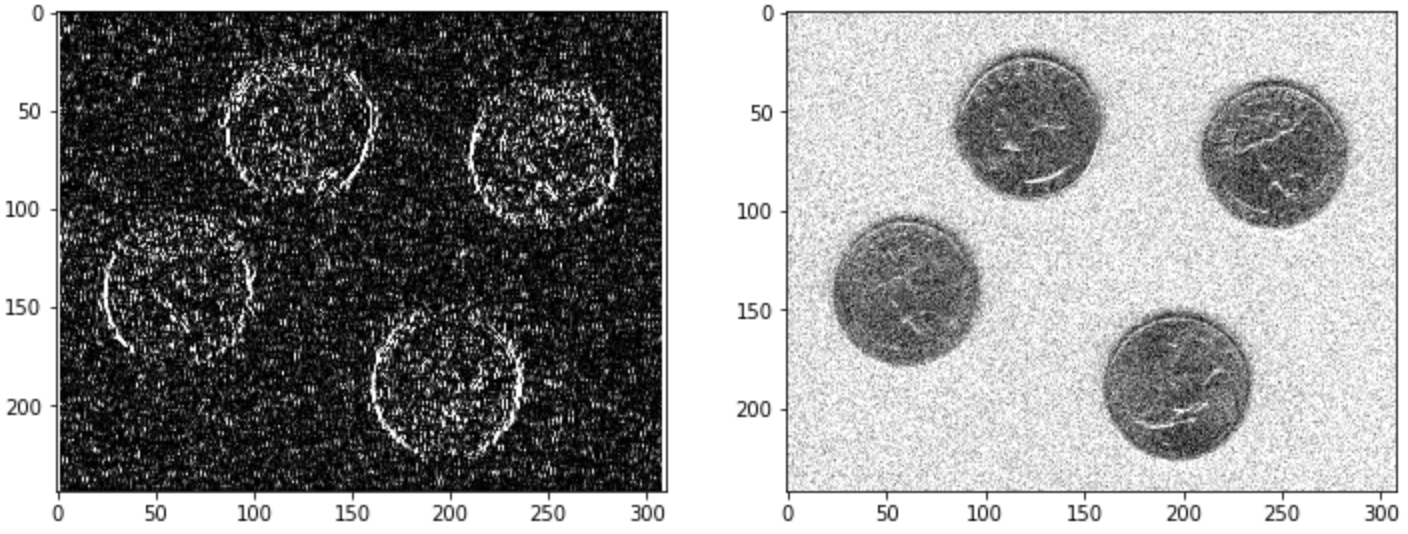
\includegraphics[width=\textwidth]{Materials/pvar015}
		\caption{Variance 0.015}
	\end{subfigure}
	\hfill
	\\
	\begin{subfigure}[b]{\textwidth}
		\centering
		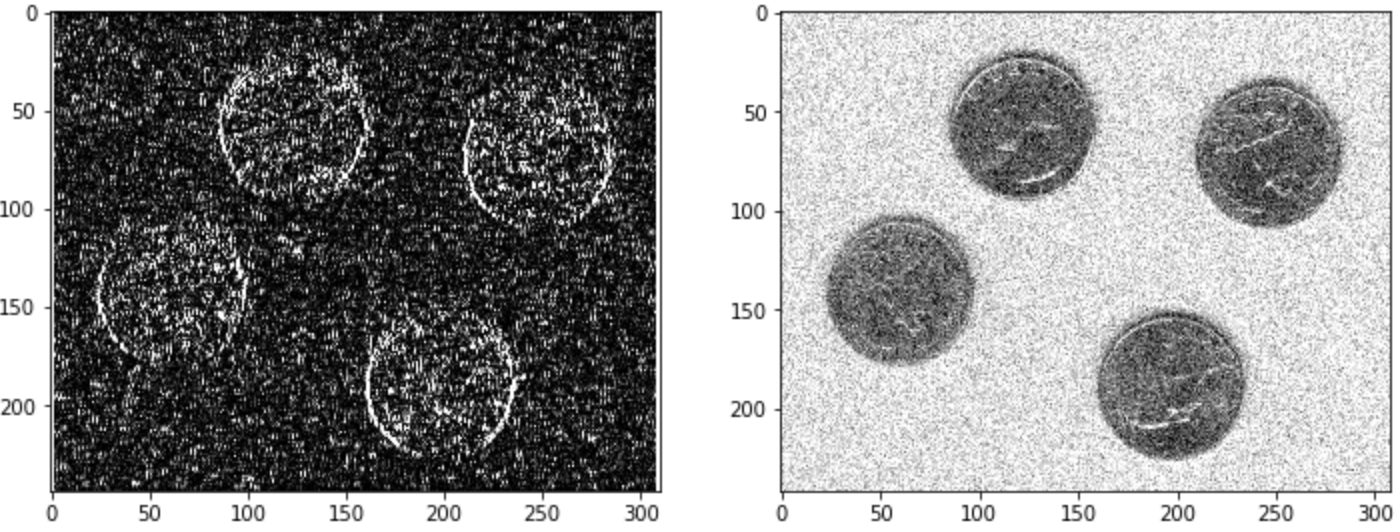
\includegraphics[width=\textwidth]{Materials/pvar02}
		\caption{Variance 0.02}
	\end{subfigure}
	\caption{Gradients produced by filtering with Prewitt.}
	\label{prewitt2}
\end{figure}
In \autoref{sobel1}, \autoref{sobel2}, \autoref{prewitt1} and \autoref{prewitt2} we see filtering with the Sobel and Prewitt filter for different variances. We see that the Prewitt filter seems to less effected by noise than the Sobel filter. Comparing the images with 0.2 variance it becomes somewhat hard to see the actual gradients with the Sobel filter whereas it is still rather clear in the Prewitt filter. However, the gradient is much more clear in the low variance images for the Sobel filter, where a lot more detail is also caught.\\
The code used for this exercise can be seen in \autoref{e1code}.
\begin{figure}[H]
	\centering
	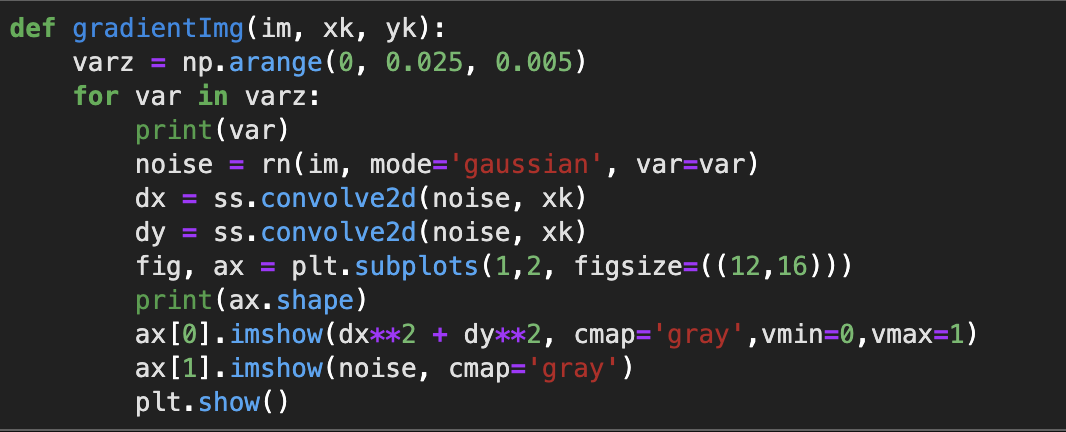
\includegraphics[width=0.7\linewidth]{Materials/e1code}
	\caption{Code for exercise 1.}
	\label{e1code}
\end{figure}
\section{Exercise 2}
\subsection*{2.1}
If we denote the pixels in the image \textit{I} as \textit{x'} and \textit{y'} and we denote the pixels in $\tilde{I}$ as \textit{x} and \textit{y}, we can map the pixels in $\tilde{I}$ to the pixels in $I$ by taking each pixel pair, \textit{x} \textit{y}, augment with a 1, and then multiply with the inverted transformation matrix:
\begin{equation*}
	\begin{bmatrix}
		x'\\
		y'\\
		1
	\end{bmatrix} = \left(
	\begin{bmatrix}
		1&0&t_x\\
		0&1&t_y\\
		0&0&1
	\end{bmatrix} \cdot
	\begin{bmatrix}
		cos(2\pi-\theta)&-sin(2\pi-\theta)&0\\
		sin(2\pi-\theta)&cos(2\pi-\theta)&0\\
		0&0&1
	\end{bmatrix} \cdot
	\begin{bmatrix}
 		s&0&0\\
 		0&s&0\\
 		0&0&1
 	\end{bmatrix} \right)^{-1}	\cdot
	\begin{bmatrix}
		x\\
		y\\
		1
	\end{bmatrix}
\end{equation*}
The resulting augmented pixel pair, \textit{x'} \textit{y'}, are then the corresponding x and y coordinates in the image $\textit{I}$. Running through all pixels in $\tilde{I}$, performing this mapping and then copying the pixel value from $I$ to $\tilde{I}$ would result in the correct transformation.\\
We can also compute the inverted transformation matrix. Multiplying the three transformation matrices results in the following matrix:
\begin{equation*}
	\begin{bmatrix}
		s\cdot cos(2\pi-\theta)&s\cdot -sin(2\pi-\theta)&t_x\\
		s\cdot sin(2\pi-\theta)&s\cdot cos(2\pi-\theta)&t_y\\
		0&0&1
	\end{bmatrix}
\end{equation*}
To invert this matrix we need to perform 4 steps. In the first step we compute the matrix of minors. That is, for each entry in turn, we ignore the current row and current column, and then compute the determinant of the remaining elements which then replaces the entry we are at in the matrix. In step two we then change sign of all the elements so we get a checkerboard pattern of positive and negative values. This is the matrix of cofactors. In step three we transpose the cofactors matrix. And in the last step we multiply all elements with $\frac{1}{det} = \frac{1}{(s\cdot cos(2\pi-\theta))^2+(s\cdot -sin(2\pi-\theta)-(s\cdot sin(2\pi-\theta)))}$. We then get the matrix:
\begin{equation*}
	\frac{1}{det} \cdot 
	\begin{bmatrix}
		s\cdot cos(2\pi-\theta)&-(s\cdot -sin(2\pi-\theta)&(s\cdot -sin(2\pi-\theta)\cdot t_y)-(s\cdot cos(2\pi-\theta)\cdot t_x)\\
		-(s\cdot sin(2\pi-\theta)&s\cdot cos(2\pi-\theta)&(s\cdot cos(2\pi-\theta)\cdot t_y)-(s\cdot sin(2\pi-\theta)\cdot t_x)\\
		0&0&(s\cdot cos(2\pi-\theta))^2-(s\cdot sin(2\pi-\theta)\cdot s\cdot -sin(2\pi-\theta))
	\end{bmatrix}
\end{equation*}

\subsection*{2.2}
\begin{figure}[H]
	\begin{subfigure}[b]{0.45\linewidth}
		\centering
		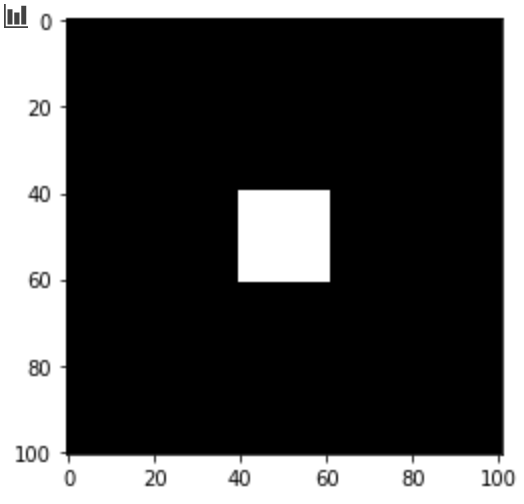
\includegraphics[width=\linewidth]{Materials/E2/before}
		\caption{Before transformation}
	\end{subfigure}
	\hfill
	\begin{subfigure}[b]{0.45\linewidth}
		\centering
		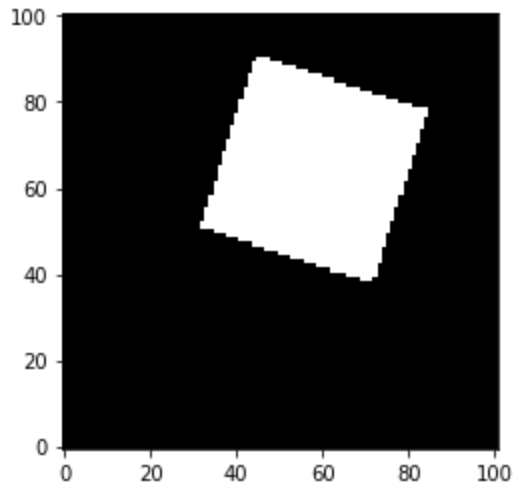
\includegraphics[width=\linewidth]{Materials/E2/res}
		\caption{After transformation}
	\end{subfigure}
	\caption{Before and after transformation of white square.}
	\label{transformation}
\end{figure}
In \autoref{transformation} we see the white square before and after the transformation. In \autoref{E2code} we see the code used for this exercise. We first define the transformation matrices in homogenous coordinates and then dot them all together, and then we take the inverse of this matrix as he final transformation matrix. We then loop through all pixels in the output image and map them to the input image through the inverted transformation matrix. To make the dotting of the transformations work, we use 3x3 matrices, and thus the input coordinates needs to be augmented with a third coordinate equal to 1. The output coordinate is also augmented, and to convert back to Cartesian coordinates we thus divide the \textit{x} and \textit{y} coordinates with the augmented output coordinate, however, this augmented output coordinate is always 1, so we simply just get the \textit{x} and \textit{y} coordinate. To accommodate the nearest neighbour interpolation, we simply round the coordinates. After we have performed the transformation, we plot the new square where we have changed the direction of the y-axis to be of correct orientation.

\begin{figure}[H]
	\centering
	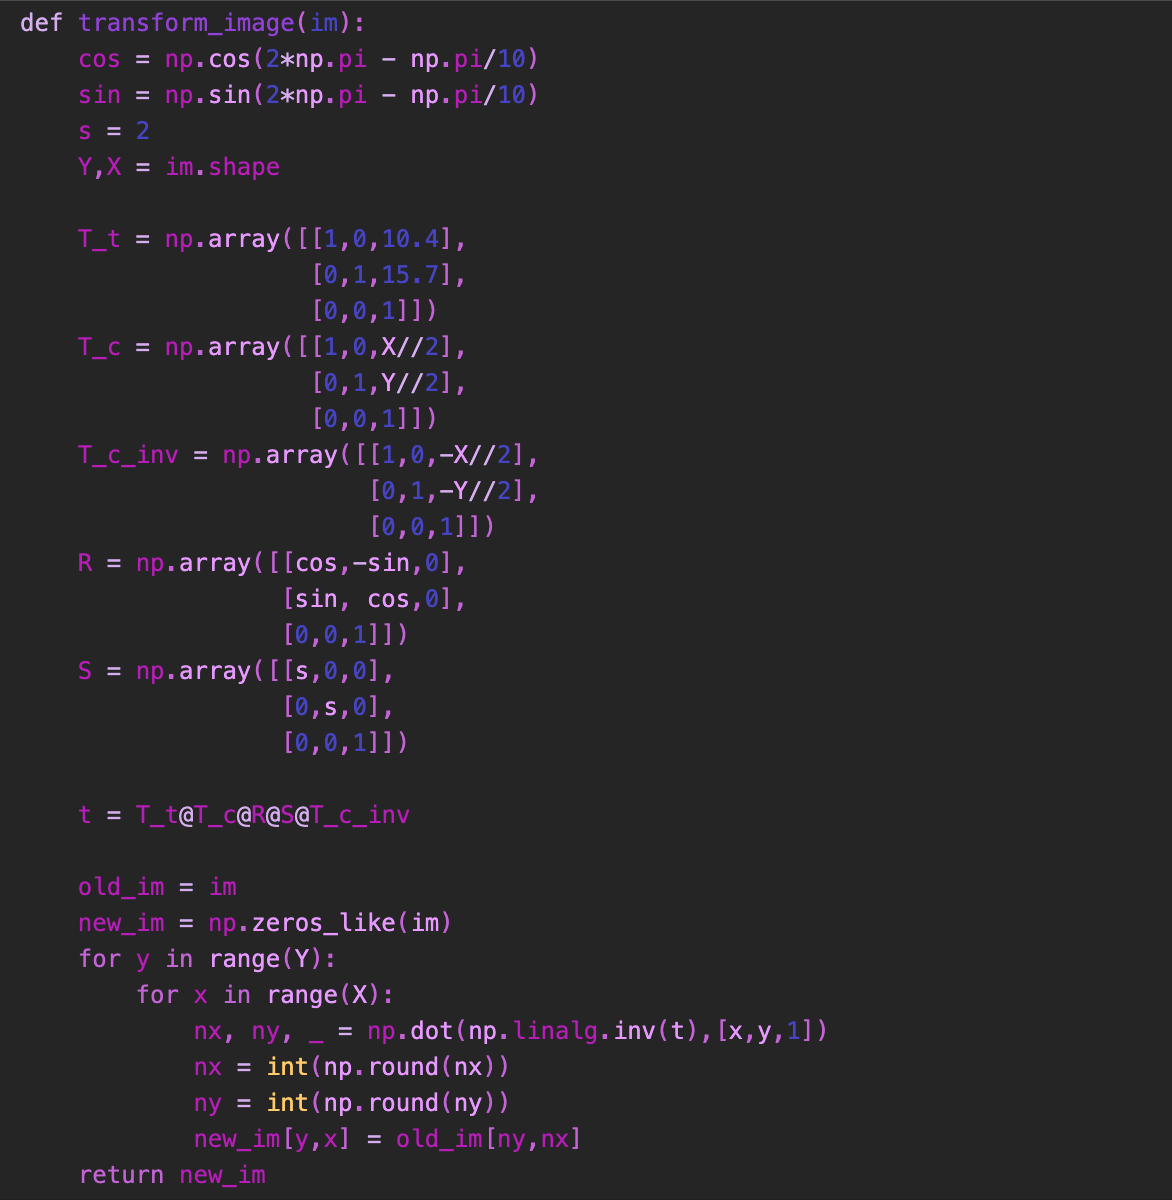
\includegraphics[width=\linewidth]{Materials/E2/code}
	\caption{Code used for this exercise.}
	\label{E2code}
\end{figure}
\section{Exercise 3}
\subsection*{3.1}
\begin{figure}[H]
	\centering
	\begin{subfigure}[b]{0.45\textwidth}
		\centering
		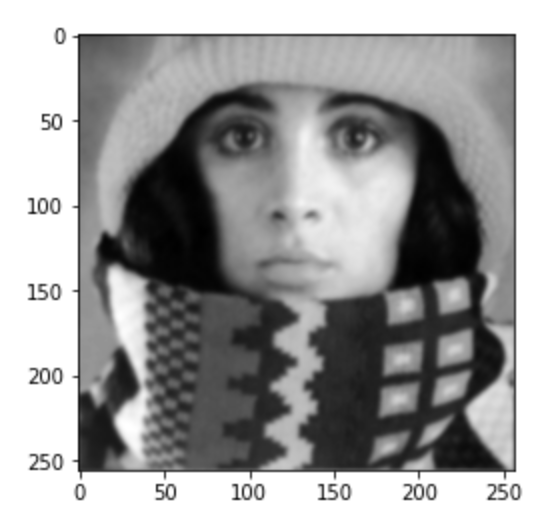
\includegraphics[width=\textwidth]{Materials/004}
		\caption{$\sigma = 0.004$.}
	\end{subfigure}
	\hfill
	\begin{subfigure}[b]{0.45\textwidth}
		\centering
		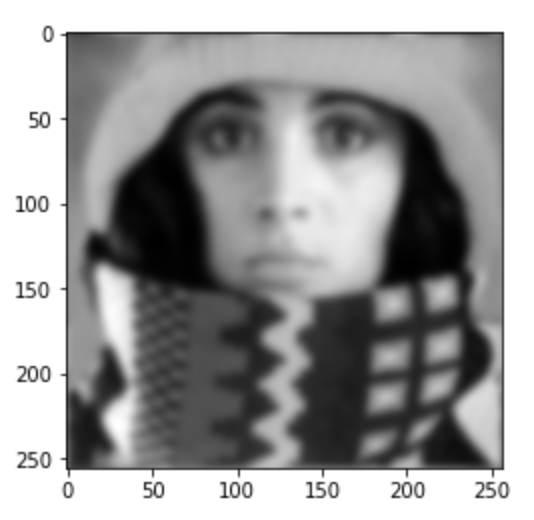
\includegraphics[width=\textwidth]{Materials/01}
		\caption{$\sigma = 0.01$.}
	\end{subfigure}
	\hfill
	\\
	\begin{subfigure}[b]{0.45\textwidth}
		\centering
		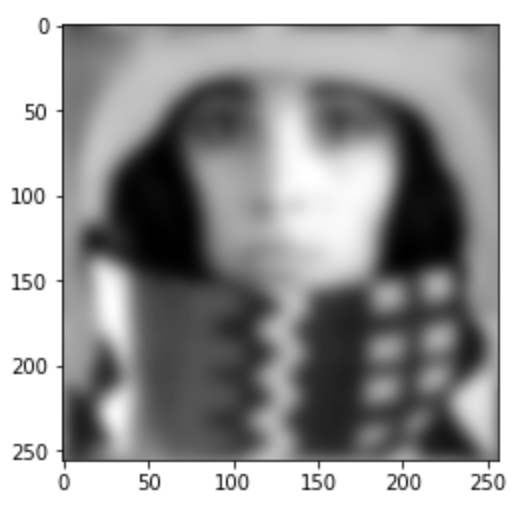
\includegraphics[width=\textwidth]{Materials/02}
		\caption{$\sigma = 0.02$.}
	\end{subfigure}
	\hfill
	\begin{subfigure}[b]{0.45\textwidth}
		\centering
		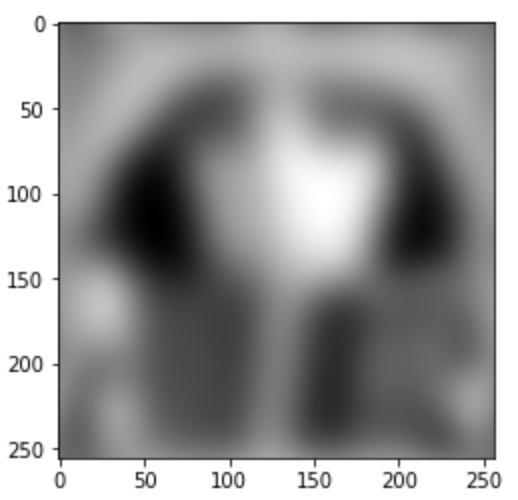
\includegraphics[width=\textwidth]{Materials/05}
		\caption{$\sigma = 0.05$.}
	\end{subfigure}
	\caption{Gaussian kernel constructed in frequency space multiplied by Fourier transform of \textit{'trui'}.}
	\label{gaussian}
\end{figure}

From the convolution theorem we know that convolution in the spatial domain is equal to multiplication in frequency domain. That is:
\begin{equation*}
		\mathcal{F}{f*g}(u) = \mathcal{F}{f}(u)\cdot \mathcal{F}{g}(u) = F(u)\cdot G(u)
\end{equation*}
Thus, if we want to perform convolution between two functions, we can instead find both functions Fourier transform, multiply these together, and then take the inverse Fourier transform of the result.\\
In \autoref{gaussian} we see the result of constructing a Gaussian kernel in frequency space and multiply it with the Fourier transform of \textit{'trui.png'} and then take the inverse Fourier transform of the result. The code used for this exercise can be seen in \autoref{e31code}. The kernel constructed by \textit{'fftgausK'} is defined based on the Fourier transform of a Gaussian kernel given in the lecture slides.
\begin{figure}[H]
	\centering
	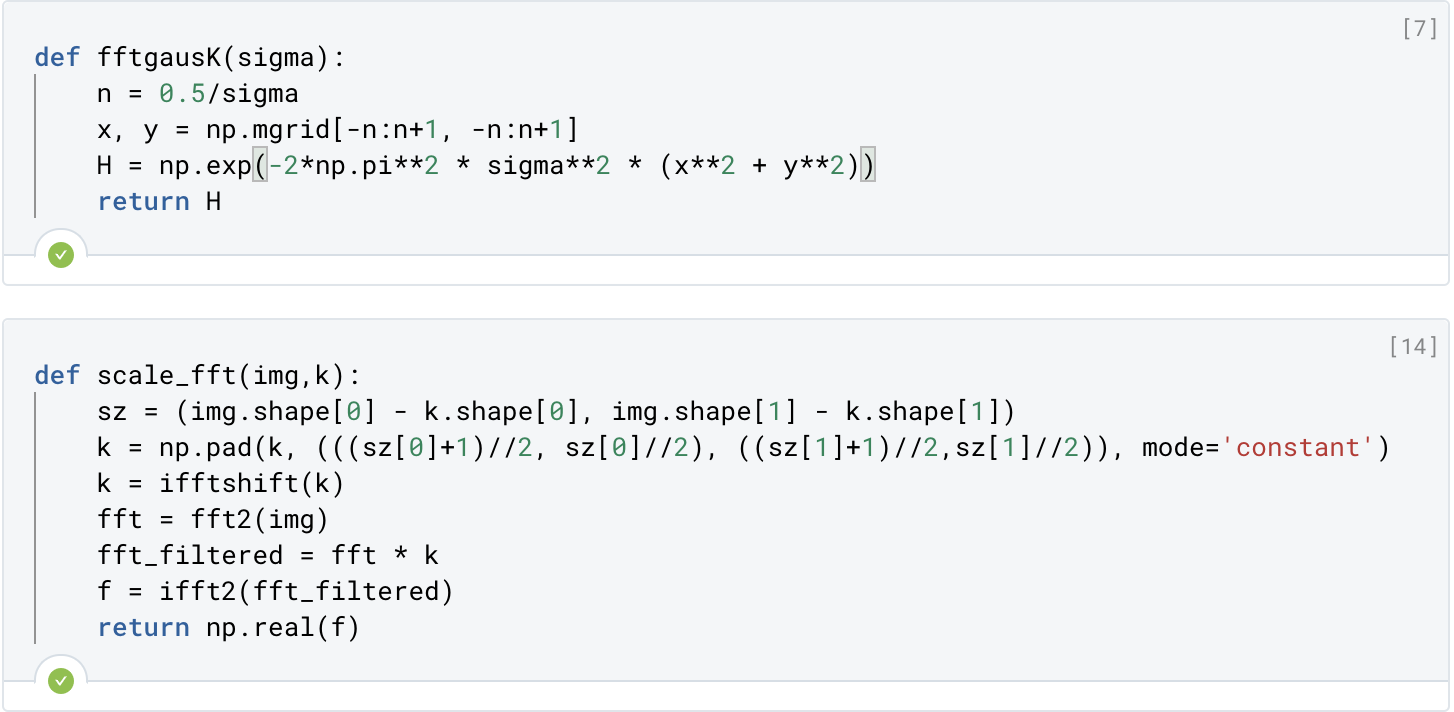
\includegraphics[width=\linewidth]{Materials/e31code}
	\caption{Code for exercise 3.1.}
	\label{e31code}
\end{figure}

\subsection*{3.2}
\begin{figure}[H]
	\centering
	\begin{subfigure}[b]{0.45\textwidth}
		\centering
		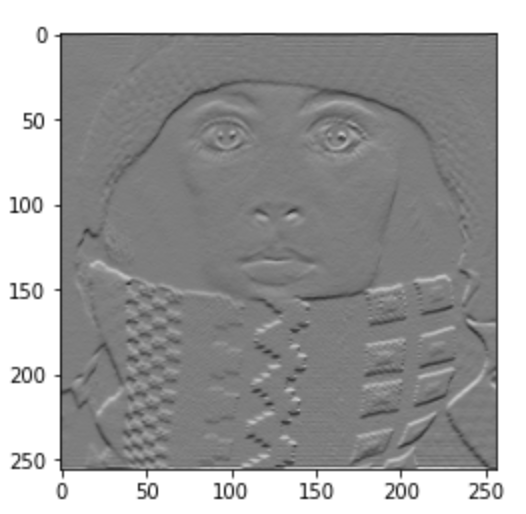
\includegraphics[width=\textwidth]{Materials/3210}
		\caption{First order y derivative.}
	\end{subfigure}
	\hfill
	\begin{subfigure}[b]{0.45\textwidth}
		\centering
		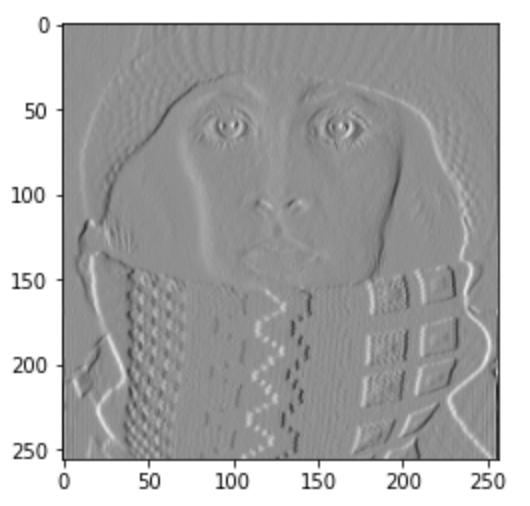
\includegraphics[width=\textwidth]{Materials/3201}
		\caption{First order x derivative.}
	\end{subfigure}
	\hfill
	\\
	\begin{subfigure}[b]{0.45\textwidth}
		\centering
		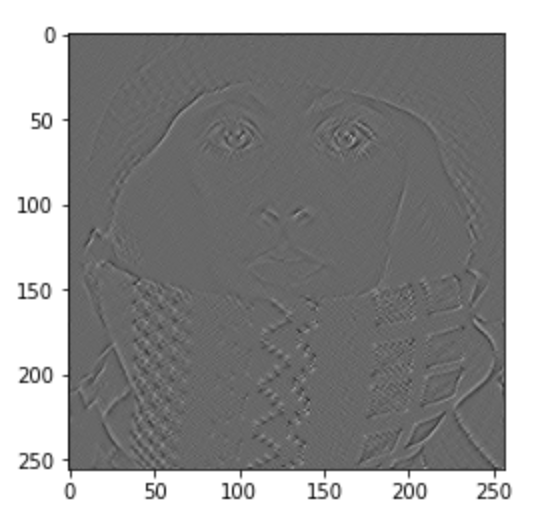
\includegraphics[width=\textwidth]{Materials/3211}
		\caption{First order x and y derivative.}
	\end{subfigure}
	\hfill
	\begin{subfigure}[b]{0.45\textwidth}
		\centering
		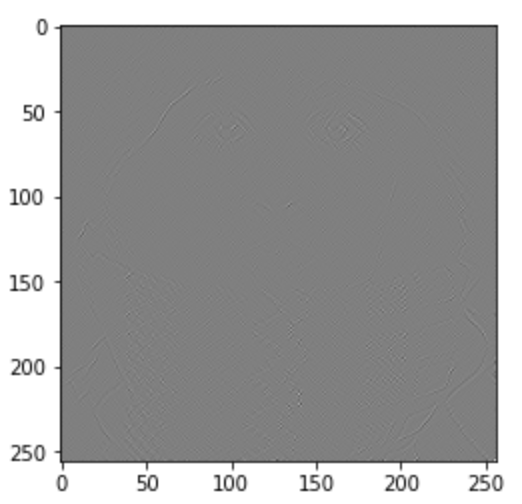
\includegraphics[width=\textwidth]{Materials/3222}
		\caption{Second order x and y derivative.}
	\end{subfigure}
	\caption{Partial derivatives of \textit{'trui'} image.}
	\label{deriv}
\end{figure}

From the lecture slides we have the derivative theorem which tells us $\frac{\partial^m}{\partial x^m}\frac{\partial^n}{\partial y^n}f(x,y)$ in spatial domain is equivalent to $(iu)^m(iv)^bF(u,v)$ in the frequency domain. That is, we can construct a kernel based on $(iu)^m(iv)^b$, multiply by $F(u,v)$ and then take the inverse Fourier transform to get our partial derivatives. The results can be seen in \autoref{deriv} and the code can be seen in \autoref{e32code}.
\begin{figure}[H]
	\centering
	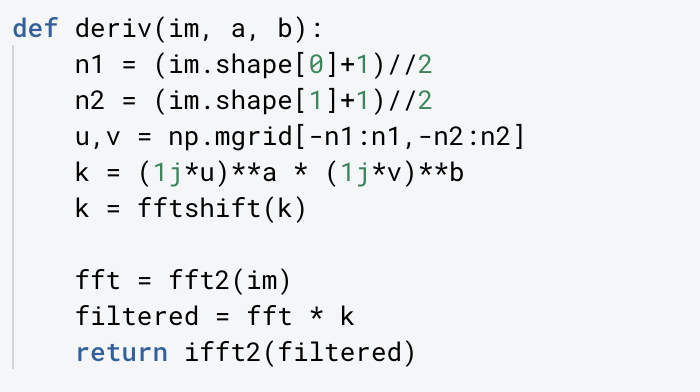
\includegraphics[width=0.7\linewidth]{Materials/e32code}
	\caption{Code for exercise 3.2.}
	\label{e32code}
\end{figure}
\section{Exercise 4}
\subsection*{4.1}
\begin{figure}[H]
	\centering
	\begin{subfigure}[b]{0.45\textwidth}
		\centering
		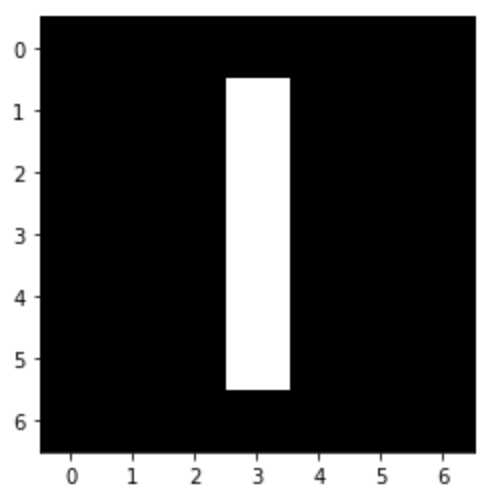
\includegraphics[width=\textwidth]{Materials/digit}
		\caption{The chosen digit / input image.}
	\end{subfigure}
	\hfill
	\begin{subfigure}[b]{0.45\textwidth}
		\centering
		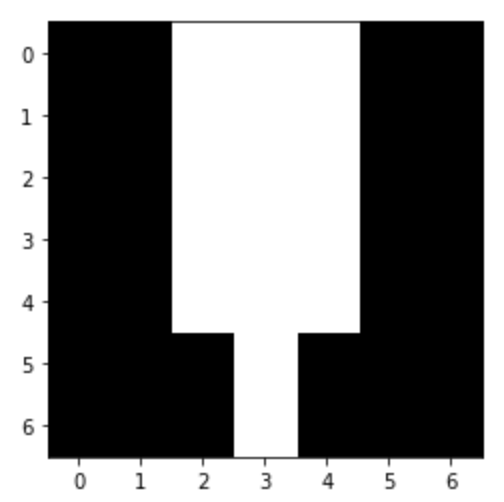
\includegraphics[width=\textwidth]{Materials/m1res}
		\caption{Dilation with mask 1.}
		\label{m1res}
	\end{subfigure}
	\hfill
	\\
	\begin{subfigure}[b]{0.45\textwidth}
		\centering
		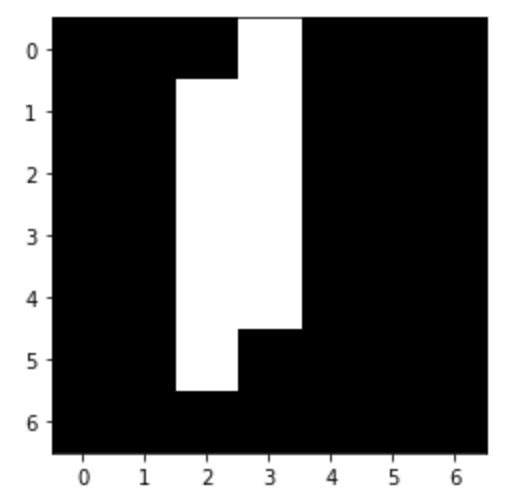
\includegraphics[width=\textwidth]{Materials/m2res}
		\caption{Dilation with mask 2.}
		\label{m2res}
	\end{subfigure}
	\hfill
	\begin{subfigure}[b]{0.45\textwidth}
		\centering
		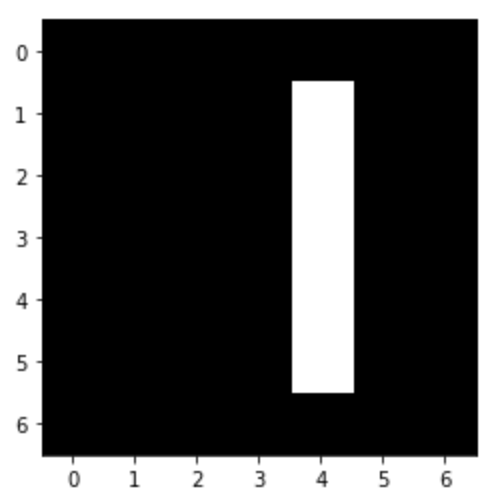
\includegraphics[width=\textwidth]{Materials/m3res}
		\caption{Dilation with mask 3.}
		\label{m3res}
	\end{subfigure}
	\caption{Results of dilation with masks from the exercise.}
\end{figure}
\textbf{i.:}The structuring element does not need to be symmetric. As can be seen in \autoref{m1res} the resulting image after dilation adds the 'T' shape to the input image. The centre pixel is defined as the middle one in the 3 by 3 grid, i.e. the white pixel in the second row.\\
\textbf{ii.:} The structuring element does not need to have an odd number of pixels in both directions. In \autoref{m2res} we see the diagonal pattern added to the input image. The centre pixel is the lower right black pixel.\\
\textbf{iii.:} The structuring element does not need to have the middle pixel set to true. As seen in \autoref{m3res} the output simply gets shifted. The centre pixel is the middle black pixel.\\
The code for this exercise can be seen in \autoref{e41code}.
\begin{figure}[H]
	\centering
	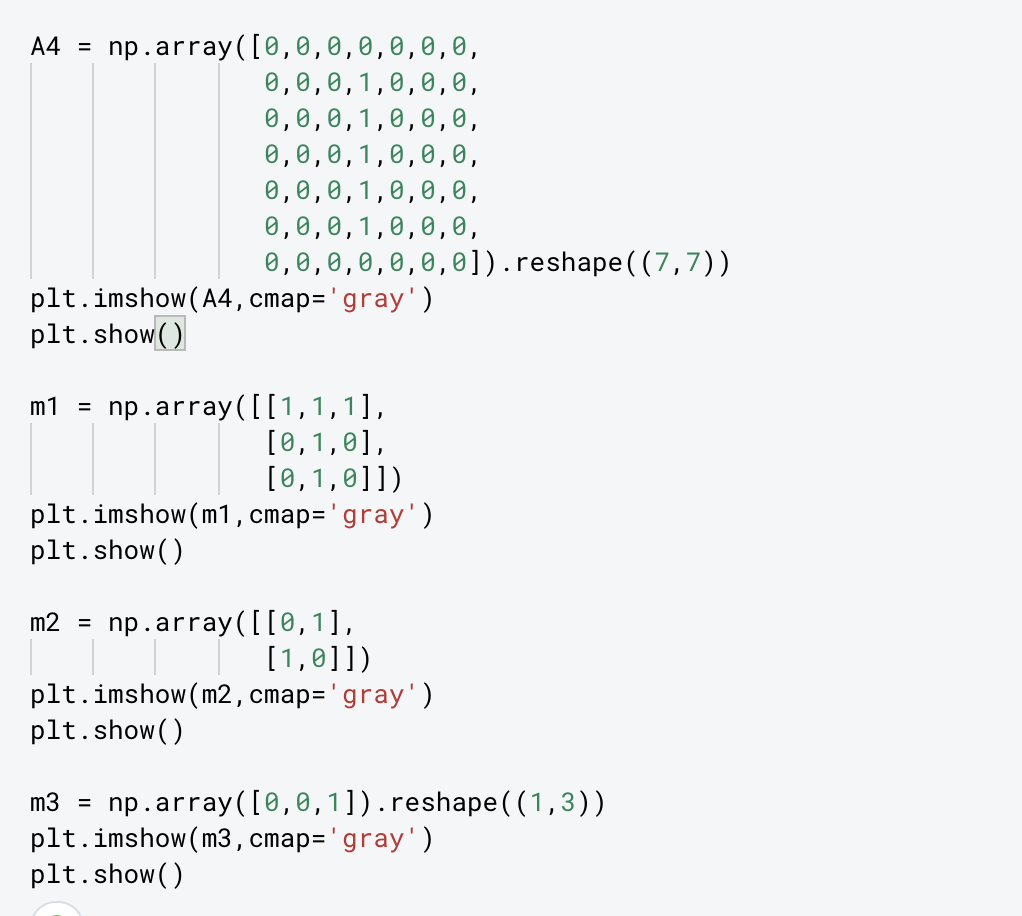
\includegraphics[width=0.7\linewidth]{Materials/e41code}
	\caption{Code for exercise 4.1.}
	\label{e41code}
\end{figure}

\subsection*{4.2}
\begin{figure}[H]
	\centering
	\begin{subfigure}[b]{0.45\textwidth}
		\centering
		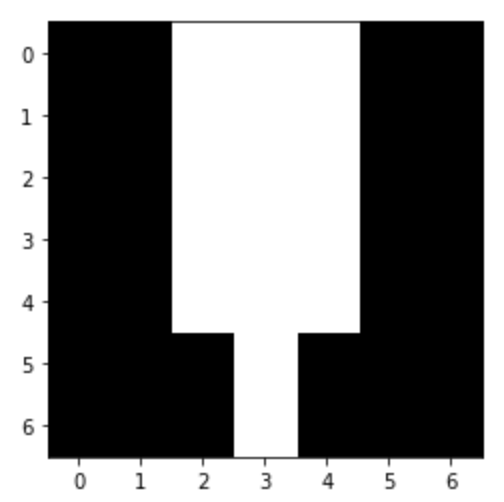
\includegraphics[width=\textwidth]{Materials/m1res}
		\caption{Mask 1.}
	\end{subfigure}
	\hfill
	\begin{subfigure}[b]{0.45\textwidth}
		\centering
		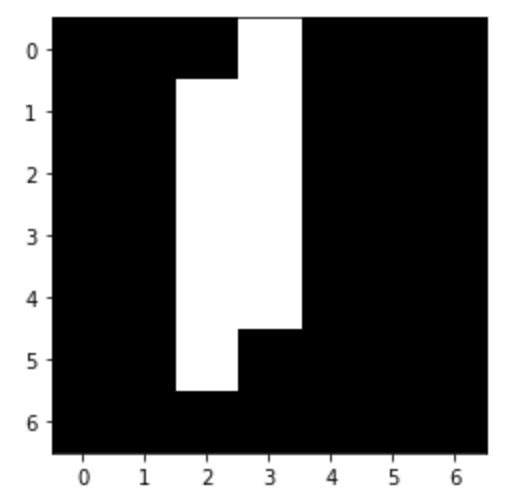
\includegraphics[width=\textwidth]{Materials/m2res}
		\caption{Mask 2.}
	\end{subfigure}
	\hfill
	\\
	\begin{subfigure}[b]{0.45\textwidth}
		\centering
		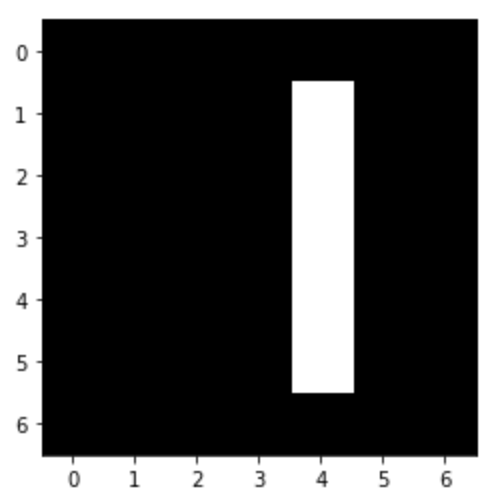
\includegraphics[width=\textwidth]{Materials/m3res}
		\caption{Mask 3.}
	\end{subfigure}
	\caption{Results of dilation of masks with input image.}
	\label{dilation}
\end{figure}
When performing the dilation with the input image on the masks we get the exact same results as before due to the commutative property of dilation. This indeed means we can interchange the input image and mask and get the same results. This can be useful if either the mask or the input image contains \textit{many} more 'true' pixels than the other, then interchanging the mask and the input image such that we only need to perform dilation on a few 'true' pixels might speed things up.\\
The results of this exercise can be seen in \autoref{dilation} and the code for this exercise can be seen in \autoref{e42code}.
\begin{figure}[H]
	\centering
	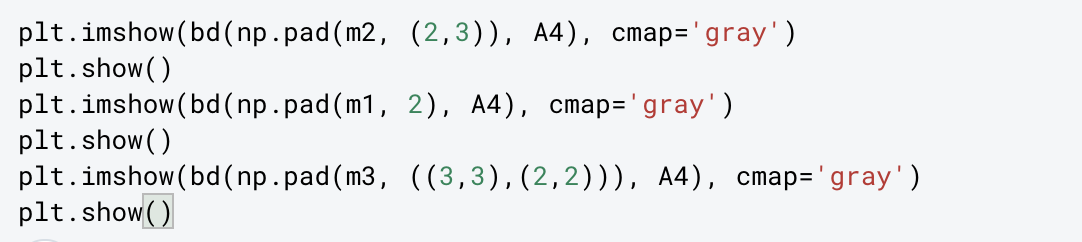
\includegraphics[width=0.7\linewidth]{Materials/e42code}
	\caption{Code for exercise 4.2.}
	\label{e42code}
\end{figure}


\end{document}